In this section we present heuristics we previously developed and applied to one kind of
distributed system: software-defined networking (SDN) control software. In~\cite{sts2014} we
empirically showed that these heuristics work well.
Here, we begin by briefly describing the behavior of SDN
control software.

\noindent {\bf Overview of SDN Control Software.} Network operating systems, the key component of SDN software
infrastructure, consist of control software running on a replicated set of
servers, each running a controller instance. Controllers coordinate between
themselves, and receive input events (\eg~link failure notifications) and
statistics from switches (either physical or virtual), policy
changes via a management interface, and possibly dataplane packets.
In response, the
controllers issue forwarding instructions to switches. All input
events are asynchronous, and individual controllers may fail at any
time. The controllers either communicate
with each other over the dataplane network, or use a separate dedicated
network, and may become partitioned.

%\subsection{Bugs, QA Testing, and Troubleshooting}
The goal of the network control plane is to configure the switch forwarding entries so as to
enforce one or more invariants, such as connectivity (\ie~ensuring that a
route exists between every endpoint pair), isolation and access control
(\ie~various limitations on
connectivity), and virtualization (\ie~ensuring that packets are handled
in a manner consistent with the specified virtual network).
A bug causes an invariant to be violated. Invariants can be
violated because the system was improperly configured
%A bug causes an invariant to be violated. Bugs can occur in the
%configuration management system, \eg~OpenStack~\cite{quantum}
(\eg~the management system~\cite{quantum} or a human improperly specified their goals), or
because there is a bug within the SDN control plane itself. In this paper we focus on troubleshooting bugs in the
SDN control plane after it has been given a policy configuration.\footnote{This does
not preclude us from troubleshooting misspecified policies
so long as test
invariants~\cite{hsa} are specified separately.}

\noindent {\bf Heuristics for Accounting for Interleavings.} To reproduce an invariant
violation found in an execution of SDN control software,
we need to inject each input event \external{} only after all other
events, including internal events,
that precede it in the
happens-before relation~\cite{Lamport:1978:TCO:359545.359563} from the
original execution ($\{i \mid i \rightarrow\!\!\text{\external{}}\}$) have
occurred~\cite{tel2000introduction}.

The internal events we consider are
(a) message delivery events, either between controllers (\eg~database
synchronization messages) or
between controllers and switches (\eg~OpenFlow messages), and (b) state transitions
within controllers (\eg~a backup node deciding to become master).
Our replay orchestrator obtains visibility into (a) by interposing on all messages within the test
environment (described in detail in~\cite{sts2014}).
It optionally obtains partial visibility into (b) by instrumenting controller
software with a simple interposition layer (described in~\cite{sts2014}).

%From the perpsective
%By virtue of managing inputs and message deliveries from a central location, we are
%able to totally-order the event trace $\tau_L$.
%We thereby augment the log $(E_L, T_L)$ with a schedule
%$\tau_L\!=\!e_1\!\rightarrow\!i_1\!\rightarrow\!\dots\!e_2\!\rightarrow\!\dots$, where
%each $i$ is an internal event observed in the original run.

\colin{Add back in (reword) if we have space:}
%Note that we do not control the occurrence of internal events, and therefore do
%not attempt to minimize them. Crucially though, we need to ensure that the ordering
%of input and internal events during
%$replay()$ of each subsequence is consistent with the happens-before relation,
%so that we can report invariant violations
%(minimization opportunities) to delta debugging as often as possible.
%To meet this requirement our test orchestrator may use its interposition on
%messages to reorder or drop messages as necessary during replay.
%The final MCS produced by our system therefore includes a schedule
%$\tau_S\!=\!e_1\!\rightarrow\!i_1'\!\rightarrow\!\dots\!e_2\!\rightarrow\!\dots$
%reflecting how the minimal subsequence of inputs should be interleaved
%with internal events in order to reproduce the invariant violation. This
%schedule supersedes the timings $T$ described in \S\ref{sec:formalism}.

%\subsection{Preserving Causality}

\begin{table}[tb]
\centering
\footnotesize
\begin{tabular}{|l|l|}
\hline
{\bf Internal Message} & {\bf Masked Values} \\
\hline
\hline
OpenFlow messages & xac id, cookie, buffer id, stats \\
% port numbers?
\hline
packet\_out/in payload & all values except src, dst, data \\
\hline
Log statements & varargs parameters to printf \\
\hline
\end{tabular}
\caption{Internal messages and their masked values. %The masks serve to
%define equivalence classes.
}
\label{tab:fingerprints}
\vspace{-0.6cm}
\end{table}

Given a subsequence $E_S$, our goal is to find an execution that obeys the
original happens-before relation. We do not control the
occurrence of internal events, but we can manipulate when they are delivered
through our interposition layer,\footnote{In this way we totally order
messages. Without interposition on process scheduling however, the
system may still be concurrent.}
and we also decide when to inject the external
events $E_S$. The key challenges in choosing a schedule stem from the fact
that the original execution has been modified: internal events may differ
syntactically, some expected internal events may no
longer occur, and new internal events may occur that were not observed at all
in the original execution.\\[0.5ex]
%
%\eat{
%\colin{Somewhat redundant. Maybe wait until use cases.}
%While the inputs and original internal events are given to us,
%we become aware of new internal events throughout replay by
%(i) monitoring
%control message receipts between controllers and switches,
%and (ii) interposing on the controllers' logging library and notifying the
%replayer whenever the control software executes a log statement (which serve to mark relevant state
%transitions). Note that to achieve truly deterministic
%replay, these log statements would need to
%be highly granular, capturing information such as thread scheduling decisions;
%we show in \S\ref{subsec:case_studies}
%however that pre-existing, course granular log statements are often sufficient to
%successfully reproduce bugs.}
%
%%\footnote{We discuss this problem further in
%%\S\ref{subsec:domain_knowledge}.}
%%Note that the developer must provide enough logging statements
%%so that relevant internal state transitions are captured and visible to our
%%tool.
%
\noindent {\bf Functional Equivalence. } Internal events may differ syntactically (\eg~sequence numbers
of control packets may all differ) when replaying a subsequence of the original log.
We observe that many internal events are {\em functionally
equivalent}, in the sense that they
have the same effect on the state of the system with respect to triggering the
invariant violation. For example,
\verb=flow_mod=
messages may cause switches to make the same change to their forwarding behavior
even if their transaction ids differ.

We apply this observation by defining
masks over semantically extraneous fields of
internal events.\footnote{One consequence
of applying masks is that bugs involving masked fields are outside the purview of
our approach.} We show the fields we mask in Table~\ref{tab:fingerprints}.
Note that these masks only need to be specified once, and can later be
applied programmatically.

\begin{table}[tb]
\centering
\footnotesize
\begin{tabular}{|l|l|}
\hline
\textbf{Input Type} & \textbf{Implementation} \\
\hline
\hline
Switch failure/recovery & TCP teardown \\
\hline
Controller failure/recovery & \verb=SIGKILL= \\
\hline
Link failure/recovery & \verb=ofp_port_status= \\
\hline
Controller partition & \verb=iptables= \\
\hline
Dataplane packet injection & Network namespaces \\
\hline
Dataplane packet drop & Dataplane interposition \\
\hline
Dataplane packet delay & Dataplane interposition \\
\hline
Host migration & \verb=ofp_port_status= \\
\hline
Control message delay & Controlplane interposition \\
\hline
Non-deterministic TCAMs & Modified switches \\
\hline
\end{tabular}
\caption{Input types currently supported by \projectname.}
\label{tab:inputs}
\vspace{-0.2cm}
\end{table}

\eat{
\begin{figure}[t]
    %\hspace{-10pt}
    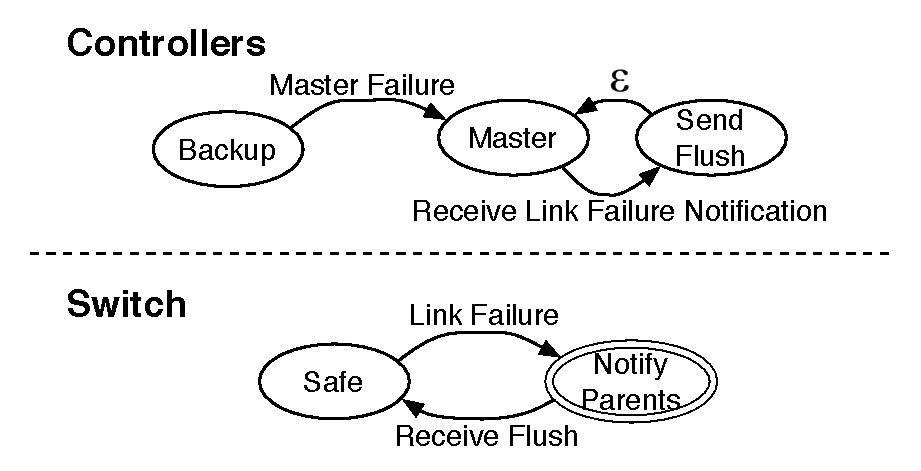
\includegraphics[width=3.25in]{../diagrams/state_machines/controller_switch.pdf}
    \caption[]{\label{fig:state_machines} Simplified state machines for the switch and
    controllers in the example Floodlight bug. Double outlined states
    represent presence of the blackhole.}
\end{figure}
}

We then consider an
internal event $i'$ observed in $replay$
equivalent (in the sense of inheriting all of its happens-before relations) to an internal
event $i$ from the original log if and only if all unmasked fields have the same value
and $i$ occurs between $i'$'s preceding and succeeding inputs in the
happens-before relation.\\[0.5ex]
%
\noindent {\bf Handling Absent Internal Events.} Some internal events from the original
log that ``happen before'' some external input
may be absent when replaying a subsequence.
For instance, if we prune a link failure,
the corresponding notification message will not arise.
\eat{
The control software's state machine (which we do not assume to know) determines whether
internal events cease to appear. Consider the simplified state machines for the switch and
controllers from the Floodlight case shown in
Figure~\ref{fig:state_machines}. If we prune the link failure input, the
master will never receive a link failure notification and
transition to and from \emph{Send Flush}.}

\eat{ % Somewhat redundant with peek()
\begin{figure}
  \footnotesize
  \begin{pseudocode}[framebox]{CausalInference}{events}
    \PROCEDURE{Replay}{subsequence}
    subsequence \GETS \CALL{Peek}{subsequence} \\
    \FOR e\textsubscript{i}\ in\ subsequence \\
      \BEGIN
      \IF e\textsubscript{i}\ is\ an\ internal\ event \\
      \AND e\textsubscript{i}\ is\ not\ marked\ absent:
      \THEN
        \BEGIN
          \Delta \GETS |e\textsubscript{i}.time - e\textsubscript{i-1}.time| + \epsilon \\
          wait\ up\ to\ \Delta\ seconds\ for\ e\textsubscript{i} \\
          \IF e\textsubscript{i}\ did\ not\ occur:
          \THEN mark\ e\textsubscript{i}\ as\ absent
        \END
      \ELSEIF e\textsubscript{i}\ is\ an\ input:
      \THEN
        \BEGIN
          \IF a\ successor\ of\ e\textsubscript{i}\ occurred: \\
          \INLINECOMMENT{waited too long}
          \THEN
            \RETURN{\CALL{Replay}{subsequence}}
          \ELSE
            inject\ e\textsubscript{i}
          \END
        \END
    \ENDPROCEDURE
  \end{pseudocode}
  \caption{{\tt Replay} is responsible for replaying subsequences of events
  chosen by delta debugging and determining
  if the bug reappears. \colin{Fix framebox width.}}
    \label{fig:replay}
\end{figure}
}

\begin{figure}
  \footnotesize
  \begin{pseudocode}[framebox]{Peek}{events}
    \PROCEDURE{Peek}{input\ subsequence}
    inferred \GETS [\ ] \\
    \FOR e\textsubscript{i}\ in\ subsequence \\
    \BEGIN
      checkpoint\ system \\
      inject\ e\textsubscript{i} \\
      \Delta \GETS |e\textsubscript{i+1}.time - e\textsubscript{i}.time| + \epsilon \\
      record\ events\ for\ \Delta\ seconds \\
      matched \GETS original\ events\ \&\ recorded\ events \\
      inferred \GETS inferred + [e\textsubscript{i}] + matched \\
      restore\ checkpoint\\
    \END \\
    \RETURN{inferred}
    \ENDPROCEDURE
  \end{pseudocode}
  \caption{{\sc Peek} determines which internal events
  from the original sequence occur for a given subsequence.
  \label{fig:peek}}
  \vskip -1.2em
\end{figure}

To avoid waiting forever we infer the presence of internal
events before we $replay$ each subsequence. Our algorithm (called {\sc Peek()}) for inferring the
presence of internal events is depicted in
Figure~\ref{fig:peek}. The algorithm injects each input, records a checkpoint\footnote{We discuss the implementation details of checkpointing
in~\cite{sts2014}.} of
the network and the control software's state, allows the system to proceed up
until the following input (plus a small time $\epsilon$), records the observed
events, and matches the
recorded events with the functionally equivalent internal events observed in
the original trace.\footnote{In the
case that, due
to non-determinism, an internal event occurs during {\sc Peek()} but does not occur
during $replay$, we time out on internal events after $\epsilon$ seconds of
their expected occurrence.}\\[0.5ex]
%
%\eat{ % Old version without peek()
%We handle this possibility by waiting for each expected internal event
%for a certain time \textepsilon. If the internal event does not occur within
%this time, we assume that it is absent and proceed. If, however, we find
%during the \textepsilon~time units we were waiting that another internal that
%happens \emph{after} our next input occurs, we know that we have waited too
%long and violated causality. In this case we need to restart the replay
%process, this time knowing which internal events in the current
%input interval are and are not going to occur before injecting the next input.
%We show our overall event scheduling algorithm
%in Figure~\ref{fig:replay}.
%}
%
\noindent {\bf Handling New Internal Events.} The last possible induced change is the occurrence of new
internal events that were not observed in the original log.
New events present multiple possibilities for where
we should inject the next input. Consider the following case:
if $i_2$ and $i_3$ are internal events observed
during $replay$ that are both in the same equivalence class as a single event $i_1$ from the
original run, we could inject the next input after $i_2$ or after $i_3$.

% TODO: figure this figure out
%\begin{wrapfigure}{c}{1.3\linewidth}
%  \centering
%  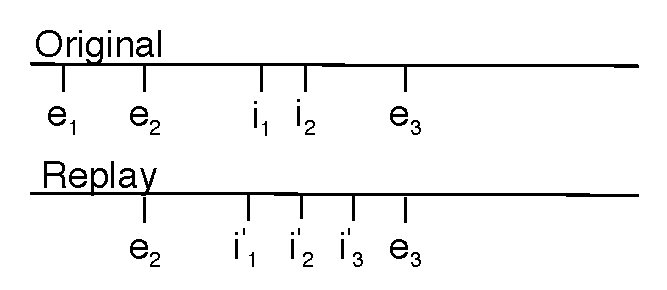
\includegraphics[width=\linewidth,height=0.8in]{../diagrams/state_machines/event_sequence.pdf}
%\end{wrapfigure}

In the general case it is always possible to construct two state machines that lead
to differing outcomes: one that only leads to the invariant violation when
we inject the next input
\emph{before} a new internal event, and another only when we inject \emph{after} a new internal
event. In other words, to be guaranteed to traverse any state transition suffix that leads
to the violation, we must recursively branch, trying both
possibilities for every new internal event. This implies an exponential worst
case number of
possibilities to be explored.

Exponential search over these possibilities is not a practical option. Our heuristic
is to proceed normally if there are new internal events,
always injecting the next input when its last expected predecessor
either occurs or times out. This ensures that we always find state transition suffixes that
contain a subsequence of the (equivalent) original internal events, but leaves open the
possibility of finding divergent suffixes that lead to the invariant
violation.\\[0.5ex]
% Cut if we need space:
%This is reasonable because not even branching on new
%internal events is guaranteed to find the globally shortest fault-inducing input
%sequence:
%there may be other unknown
%paths through the state machine leading to the invariant violation that are
%completely disjoint from the original execution.
%
%\eat{
%Luckily, crucially ambiguous new internal events are not problematic for the
%control software we evaluated, as we show in \S\ref{sec:casestudies}.
%We conjecture that ambiguous new internal events are
%rare because SDN software is a control plane system,
%and is designed to quiesce quickly (\ie~take a small number of internal
%transitions after any input event, and stop at highly connected vertices).
%Concretely, SDN programs are often structured as (mostly independent) event
%handlers, meaning that pruning input events simply triggers a subset of the original
%event handlers.
%\eat{
%As an illustration, consider the state machines
%in Figure~\ref{fig:state_machines}:
%the controllers quickly converge to a single state (either ``Master'' or
%``Backup''), as do the switches (``Safe'').
%}
%}
%
\noindent {\bf Recap.} We combine these heuristics to replay each
subsequence chosen by delta debugging: we compute functional equivalency
for all internal events intercepted by our test orchestrator's
interposition layer, we invoke {\sc Peek()} to infer absent internal events,
and with these inferred causal dependencies we $replay$
the input subsequence, waiting to inject each input until each of its
(functionally equivalent) predecessors have occurred while allowing
new internal events through the interposition layer immediately.
In~\cite{sts2014} we
empirically showed that these heuristics work well for
minimizing test cases.
